\documentclass[12pt]{scrartcl}
\usepackage[german, ngerman]{babel}
\usepackage{graphicx}
\usepackage{color}
\usepackage{url}
\usepackage{xcolor}
\usepackage{listings}
\usepackage{hyperref}
\usepackage{nameref}
\usepackage{varioref}
\hypersetup{
    colorlinks=true,
    linkcolor={black!50!black},
    % linkcolor={red!50!black},
    citecolor={black!50!black},
    urlcolor={black!50!black}
}
\usepackage[headsepline,footsepline]{scrlayer-scrpage}
\usepackage{biblatex}
\usepackage{amsmath}
\usepackage{float}

\newcommand{\code}[1]{\texttt{#1}}


\definecolor{mGreen}{rgb}{0,0.6,0}
\definecolor{mGray}{rgb}{0.5,0.5,0.5}
\definecolor{mPurple}{rgb}{0.58,0,0.82}
\definecolor{backgroundColour}{rgb}{0.95,0.95,0.95} %{cmyk}{0.05,0.05,0.05,0.05}

\lstdefinestyle{CStyle}{
    backgroundcolor=\color{backgroundColour},
    commentstyle=\color{mGreen},
    keywordstyle=\color{blue},
    numberstyle=\tiny\color{mGray},
    stringstyle=\color{mPurple},
    basicstyle=\footnotesize,
    breakatwhitespace=false,
    breaklines=true,
    captionpos=b,
    keepspaces=true,
    numbers=left,
    numbersep=5pt,
    showspaces=false,
    showstringspaces=false,
    showtabs=false,
    tabsize=2,
    language=C++
}

\lstdefinestyle{Terminal}{
    backgroundcolor=\color{backgroundColour},
    commentstyle=\color{black},
    keywordstyle=\color{black},
    numberstyle=\tiny\color{black},
    stringstyle=\color{black},
    basicstyle=\footnotesize,
    breakatwhitespace=false,
    breaklines=true,
    captionpos=b,
    keepspaces=true,
    numbers=none,
    numbersep=5pt,
    showspaces=false,
    showstringspaces=false,
    showtabs=false,
    tabsize=2,
}


\pagestyle{scrheadings}
\clearscrheadfoot
%\cfoot{Tobias Gruber}
\cfoot{\pagemark}
\chead{\headmark}
\automark[subsection]{section}


\begin{document}


\begin{titlepage}
    \vfill
	\centering

    \vspace{1.5cm}

	{\scshape\LARGE Hochschule München \par}
    {\scshape\Large Fakultät für Informatik und Mathematik\par}
	\vspace{1.5cm}




    \vfill
    {\LARGE\bfseries Praktikumsaufgabe 1 \\}
    \vspace{0.5cm}
	{in der Vorlesung\\}
    \vspace{0.5cm}
    {\LARGE\bfseries Computational Geometry\\~\\ \par}
	{\LARGE Bestimmung von Schnittpunkten aus einem gegebenen Satz von Strecken\\~\\ \par}
	\vfill
    \vfill


    \begin{tabular}{ll}
    \normalsize
    Team:  & Christopher Hinz, Tobias Gruber\\
    Studiengruppe: & Master Informatik\\
    Studiensemester: & 1. Semester\\
    Schwerpunkt: & Embedded Computing\\
    \end{tabular}
    \vspace{1.5cm}

    11.04.2022

    \vspace{0.5cm}

    Sommersemester 2022

	\vfill

\end{titlepage}

\newpage

\raggedright

%%%%%%%%%%%%%%%%%%%%%%%%%%%%%
% Problemstellung
%%%%%%%%%%%%%%%%%%%%%%%%%%%%%

\section{Einführung}
Im Rahmen der Vorlesung Computational Geometry lautet die Aufgabe für das erste Praktikum, die Anzahl der Schnittpunkte aus einem Satz von Strecken zu ermitteln.
Dafür werden 3 Dateien zur Verfügung gestellt, die jeweils Datensätze zu 1001, 10.001 und 100.001 Strecken enthalten.

Die Dateien enthalten jeweils 4 Koordinaten pro Zeile, welche jeweils die x- und y-Koordinaten eines Start- bzw. Endpunkts einer Strecke darstellen.
Die Dateien sollen jeweils eingelesen und die Anzahl der sich schneidenden Strecken durch paarweises Testen ermittelt werden.
Zusätzlich wird die aufgewendete Zeit zur Ermittlung der Anzahl der Schnittpunkte für jede Datei gemessen.

Im folgenden Abschnitt wird darauf eingegangen, wie die Grundstruktur der Problemlösung aufgebaut ist und wie die mathematische Strategie zur Lösung des Problems in C++ formuliert werden kann.
Anschließend werden die Ergebnisse der Datenauswertung vorgestellt
Es ist zu begründen, warum die Anzahl der vom Programm jeweils gefundenen Schnittpunkte korrekt ist.

\section{Abschätzung der zu erwartenden Größenordnung des Ergebnisses}

Um einschätzen zu können, inwiefern die Ergebnisse sinnvoll sind, sollen an dieser Stelle einige Vorüberlegungen getroffen werden.\\~\\
Welche Anzahl an Schnitten sind zu erwarten bzw. in welchem Wertebereich sollten sich die Ergebnisse bewegen?\\
Die minimal zu erwartende Anzahl an Schnitten wäre für 1.000, 10.0000 und 100.000 Strecken jeweils null.
Dies ist somit die untere Grenze des zu erwartenden Wertebereichs.
Die maximale Anzahl an Schnitten würden in dem Fall auftreten, dass sich alle Strecken gegenseitig schneiden.
Dann wäre nämlich für jede Strecke ein Schnittpunkt mit allen anderen Strecken gegeben.
Das Problem ist in der Mathematik auch als Sektglasproblem bekannt.
Die Berechnung erfolgt in Anlehnung an die Formel für die Dreieckszahlen.
Für eine Anzahl von n Strecken ergeben sich somit k Schnittpunkte wie folgt:
\begin{equation}
k = \frac{(n-1) \cdot n}{2}
\end{equation}
Damit wären für 1.000 Strecken maximal $499.500$ (für 10.000 maximal $49.995.000$,
für 100.000 maximal $4.999.950.000$) zu erwarten.
Dies ist somit die obere Grenze des zu erwartenden Wertebereichs.

\section{Ergebnisse der Schnittstellenberechnung und der Zeitmessung}

Das Programm verwendet die Funktion \code{read\_dat()} um die Daten aus den Dateien einzulesen und über \code{pack\_koords()} die Datensätze zu Strecken zusammenzufassen.
Jede Strecke wird anschließend gegen alle anderen Strecken geprüft, ob sie diese schneidet, oder nicht.
Zur Feststellung, ob sich die zwei Strecken schneiden wird ausgewertet, ob die Punkte $p_1, p_2$ der ersten Strecke zu den Punkten $p_1, p_2$ der zweiten Strecke im oder gegen den Uhrzeigersinn angeordnet sind.
Dafür wird folgende Formel verwendet, die im Ergebnis den Betrag des Kreuzproduktes aus den Richtungsvektoren der drei Punkte enthält:
\begin{equation}
    ccw(p, q, r) := \begin{vmatrix} p_1 & p_2 & 1 \\ q_1 & q_2 & 1 \\ r_1 & r_2 & 1 \end{vmatrix} = (p_1q_2 - p_2q_1) + (q_1r_2 - q_2r_1) + (p_2r_1 - p_1r_2)
\end{equation}

Ist das Produkt der ccw-Funktion der ersten Strecke mit den Endpunkten der zweiten Strecke, sowie das Produkt der ccw-Funktion der zweiten Strecke mit den Endpunkten der ersten Strecke kleiner oder gleich 0, so kann unter der Annahme, dass die Strecken nicht kollinear zueinander sind davon ausgegangen werden, dass sich die Strecken schneiden.

Sind die Strecken Kollinear angeordnet, so ergeben beide Kreuzprodukte 0. In diesem Fall muss noch überprüft werden, ob sich die Strecken überlappen.
Bei Überlappung der Strecken lässt sich mindestens einer der Endpunkte der zweiten Strecke über ein Vielfaches zwischen 0 und 1 des ersten Streckenvektors addiert mit einem Endpunkt der ersten Strecke darstellen.
Da zuvor bereits festgestellt wurde, dass die Strecken kollinear sind, kann der Skalar zum Richtungsvektor der zweiten Strecke über das Auflösen der parametrischen Darstellung durch die x-Komponenten der Ortsvektoren aufgelöst werden.
\begin{equation}
    \lambda = \frac{x_r - x_p}{x_q - x_p}
\end{equation}
Liegt der Wert von $\lambda$ zwischen 0 und 1, so überlappen sich die Funktionen. Nimmt $\lambda$ den Wert 0 oder 1 an, schneiden sich die Strecken in jeweils einem der Endpunkte.


In \autoref{lst:ausgabe_strecken} wird die Ausgabe des Programmes zur Schnittpunktezählung aufgeführt.
In der Ausgabe ist zu erkennen, dass die Anzahl der Schnitte für alle Fälle (1.000, 10.000, 100.000) im zu erwartenden Wertebereich liegt.
Schnittpunkte:
\begin{itemize}
    \item 1.000 Strecken: $0<= 11 <= 499.500$
    \item 10.000 Strecken: $0<= 732 <= 49.995.000$
    \item 100.000 Strecken: $0<= 77.126 <= 4.999.950.000$
\end{itemize}

% Ausgabe: strecken.cpp
\begin{lstlisting}[style=Terminal, caption={strecken.cpp: Ausgabe Konsole},captionpos=b, label={lst:ausgabe_strecken}]
# s_1000_1.dat
Strecken insgesamt: 1001
Schnitte zweier Strecken: 11
Runtime: 40.965 ms
#s_10000_1.dat
Strecken insgesamt: 10001
Schnitte zweier Strecken: 732
Runtime: 3984.3 ms
#s_100000_1.dat
Strecken insgesamt: 100001
Schnitte zweier Strecken: 77126
Runtime: 394721 ms
\end{lstlisting}


\section{Verifikation und Validierung}
Um die korrekte Funktionsweise des Programmes zu verifizieren werden verschiedene Testfälle definiert.
Die Testfälle decken unterschiedliche Streckenanordnungen ab und sollen dadurch die in der Vorlesung besprochenen Grenzfälle für Streckenschnitte überprüfen.
\autoref{fig:test_cases} zeigt die implementierten Testfälle.


% Testfälle
\begin{figure}[ht]
    \graphicspath{ {./pictures/} }
    \centering
    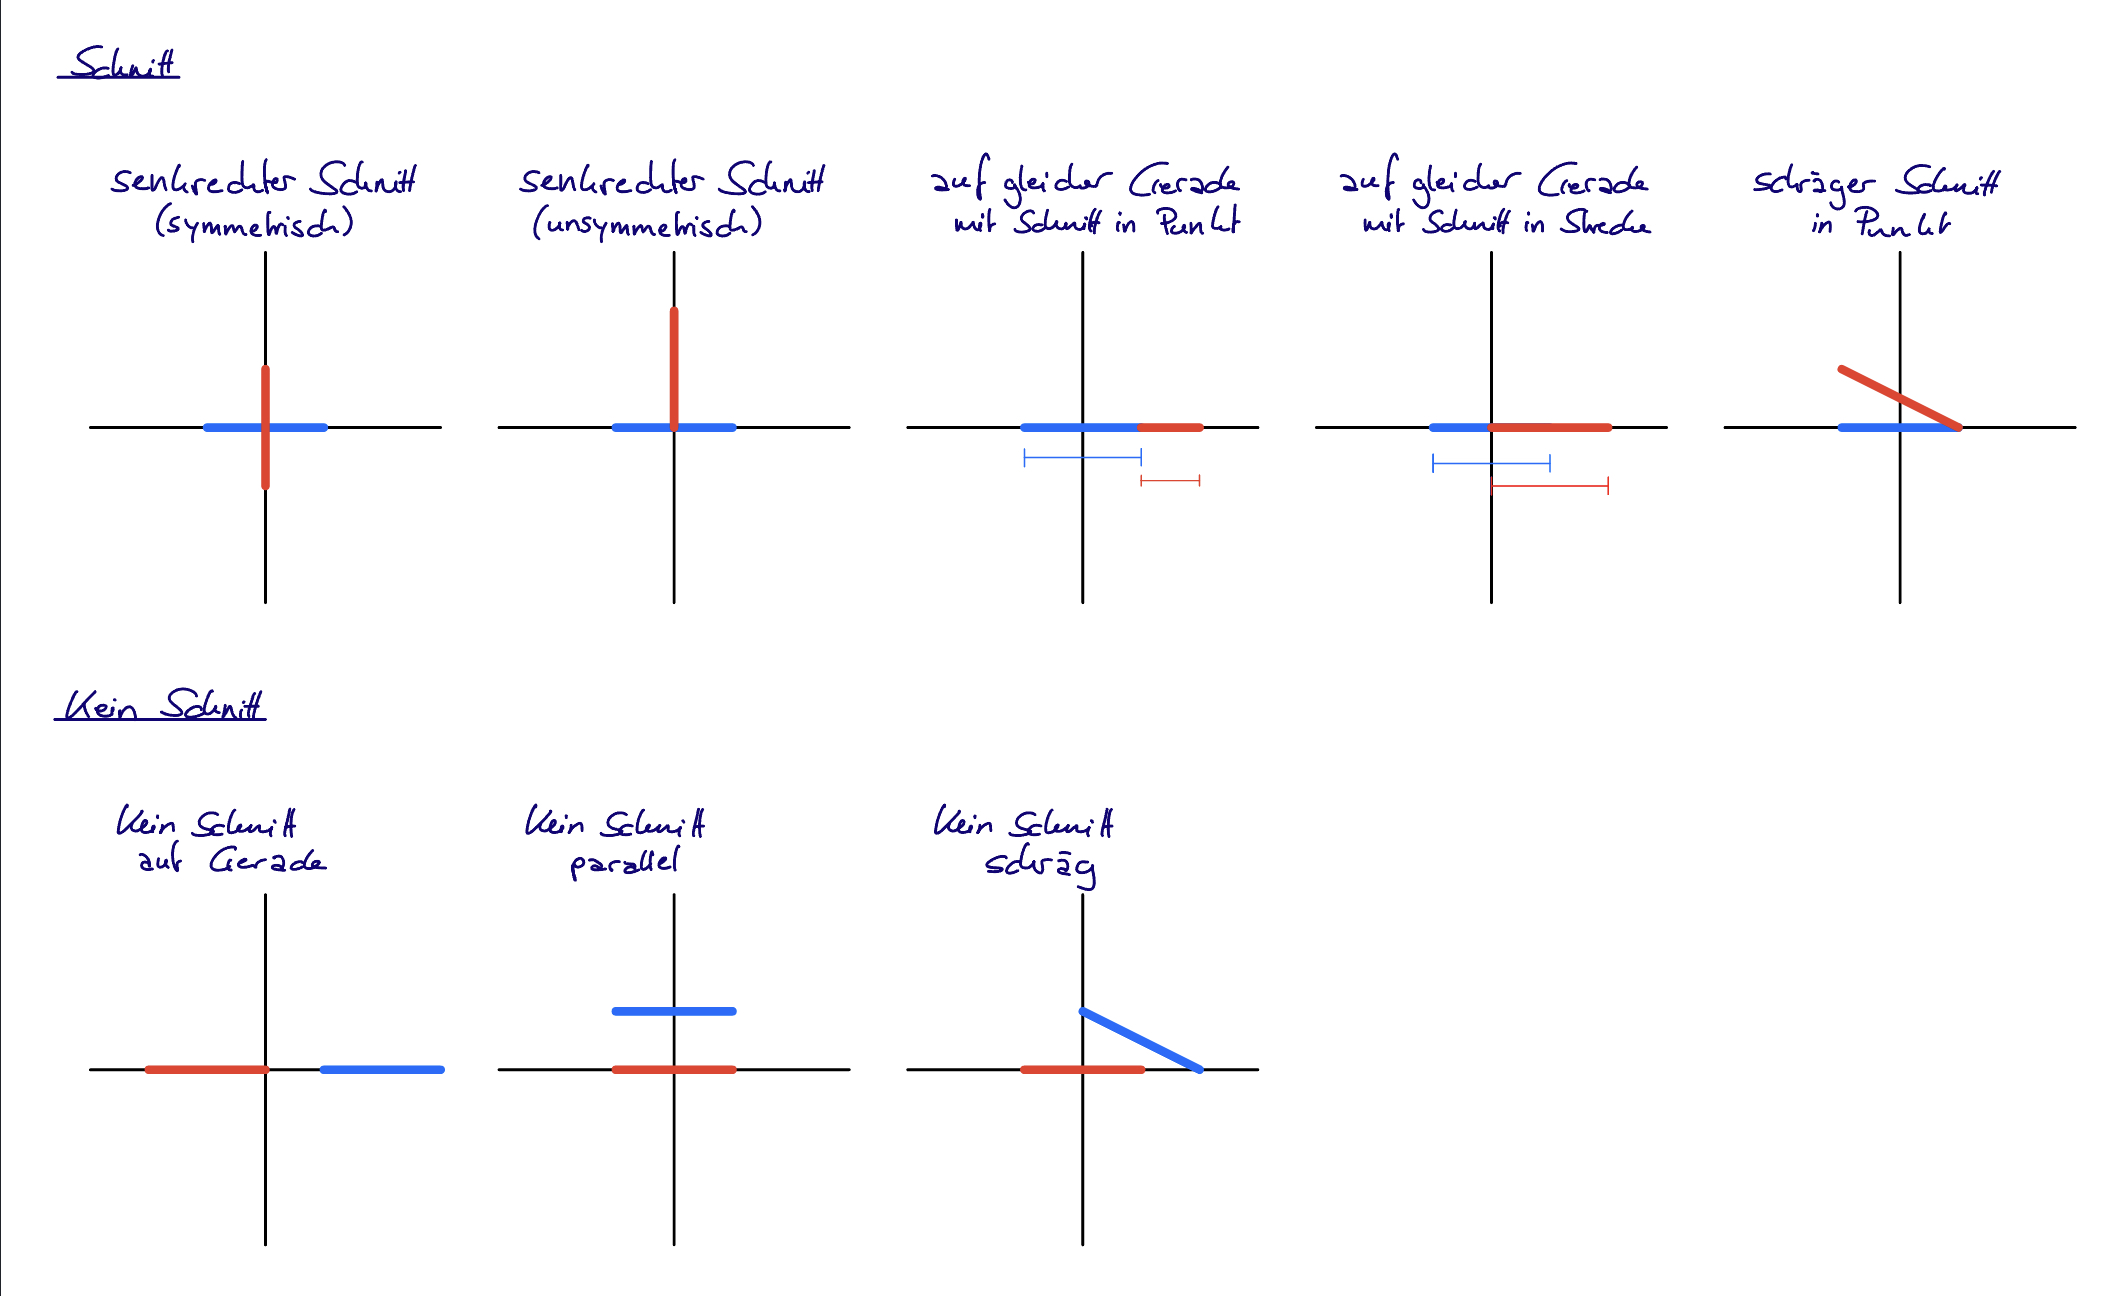
\includegraphics[scale=0.2]{Test_Vorlage.jpeg}
    \smallskip
    \caption{Testfälle für Streckenschnitte}
    \label{fig:test_cases}
\end{figure}


\ \\~\\
\autoref{lst:ausgabe_test} zeigt, dass für die Testfälle die erwarteten Ergebnisse erzielt werden.
Das bedeutet, dass für alle Streckenpaare, die wie in den Testfällen angeordnet sind, die Schnittstellenfunktion korrekt berechnet ob sie sich schneiden oder nicht.\\

\begin{lstlisting}[style=Terminal, caption={testing.cpp: Ausgabe Konsole},captionpos=b, label={lst:ausgabe_test}]
Soll: true, Ist: true
Soll: true, Ist: true
Soll: true, Ist: true
Soll: true, Ist: true
Soll: true, Ist: true
Soll: false, Ist: false
Soll: false, Ist: false
Soll: false, Ist: false
\end{lstlisting}

\ \\
Des weiteren wurde ein Python-Programm geschrieben. Dieses plottet die Strecken mit Schnittpunkten und stellt damit eine weitere Möglichkeit dar die Ergebnisse zu überprüfen.
Dies Graphen werden mittels matplotlib erstellt und sehen wie nachfolgend dargestellt aus. Auf Implementierungsdetails soll an dieser Stelle verzichtet werden, da dieses Programm ausschließlich zur Überprüfung dient.
Stichprobenartige Überprüfungen der Schnittpunkte mit diesem Programm sind alle positiv ausgefallen.

\begin{figure}[ht]
    \graphicspath{ {./pictures/} }
    \centering
    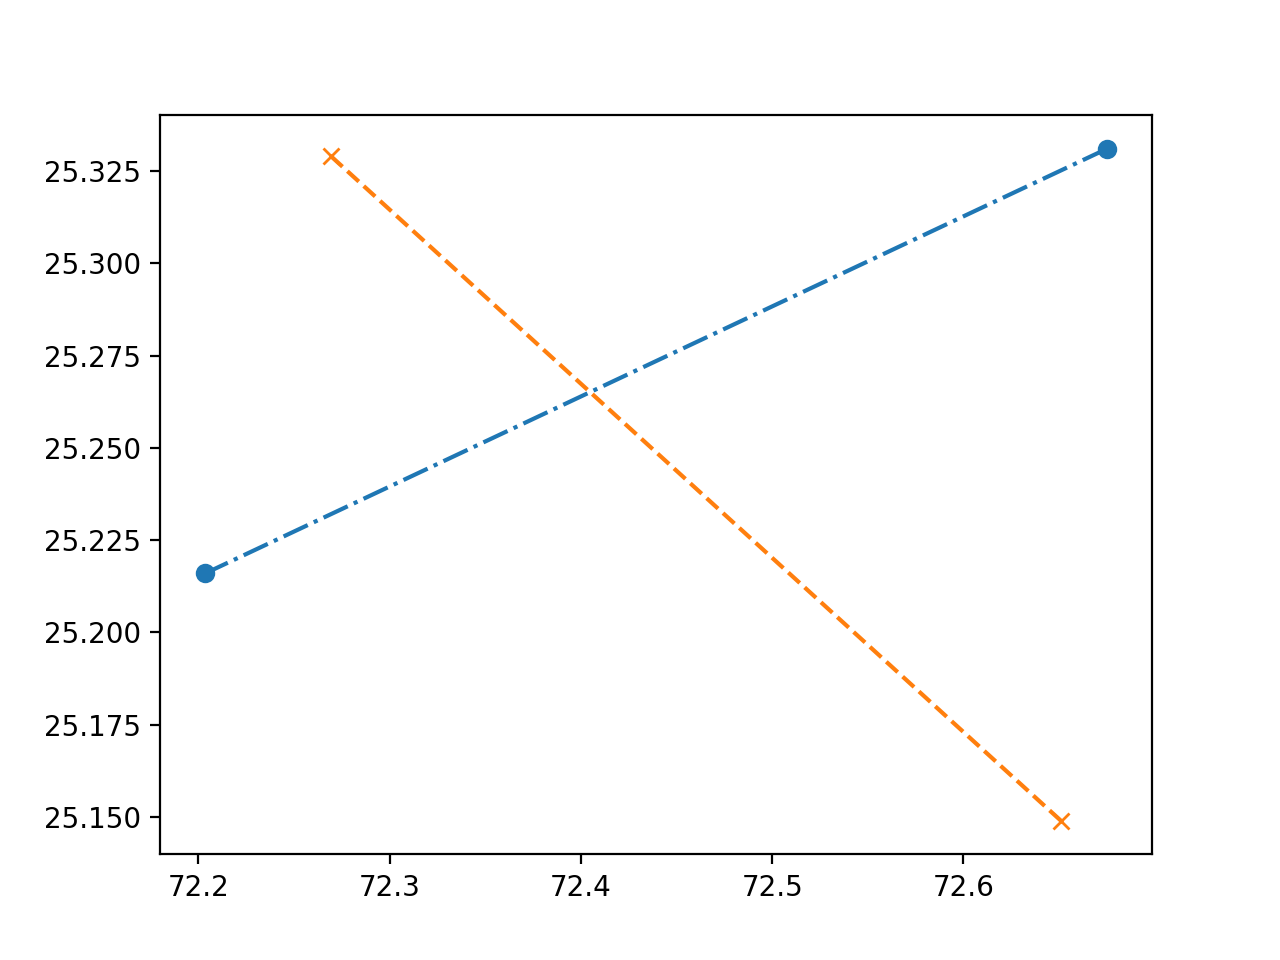
\includegraphics[scale=0.8]{python_plot1.png}
    \smallskip
    \caption{Python-Plot mit matplotlib}
    \label{fig:python_plots}
\end{figure}

Zur Validierung der Ergebnisse wurde Rücksprache mit anderen Gruppen gehalten.
Diese haben die gleichen Ergebnisse für die Anzahl der Schnittpunkte erhalten.
Zusätzlich zu der durchgeführten Verifikation ist dies ein weiteres Indiz, dass die Ergebnisse mit hoher Wahrscheinlichkeit korrekt ausfallen.

\end{document}
